\documentclass[a4paper,12pt]{report}

\usepackage{tabularx}
\usepackage{alltt, fancyvrb, url}
\usepackage{graphicx}
\usepackage[utf8]{inputenc}
\usepackage{float}
\usepackage{hyperref}
\usepackage{caption}


% Questo commentalo se vuoi scrivere in inglese.
\usepackage[italian]{babel}

\usepackage[italian]{cleveref}

% Centra verticalmente i contenuti delle righe
\renewcommand\tabularxcolumn[1]{m{#1}}


\title{\textbf{Elaborato per il corso Basi di dati}
Progettazione di una base di dati per la gestione di video perizie}


\author{
\\Buizo Manuel
\\Matteini Mattia
\\Paganelli Alberto
}
\date{\today}


\begin{document}

\maketitle

\tableofcontents

\chapter{Analisi dei requisiti}

Si vuole realizzare un database a supporto della gestione di video perizie (perizie a distanza tramite videochiamata) effettuate per varie assicurazioni italiane.
\\
La base di dati dovrà immagazzinare informazioni relativo a tutto l’ambito assicurativo, dalle assicurazioni, agli studi peritali che effettueranno le perizie.
\\
Si dovrà tenere conto anche di polizze, assicurati, dipendenti, documenti relativi alle video-perizie.


\section{Intervista }

Si vuole tenere traccia di tutte le video-perizie effettuate, di ogni studio peritale e delle parti coinvolte. 
\\
Ogni assicurazione dovrà generare sinistri di varia natura (R.C.A., Furto, Incendio, ecc…).
\\
Questi verranno assegnati agli studi, i quali si occuperanno di portare a termine le attività peritali.
\\
Ogni studio peritale dispone di un supervisore che avrà il compito di ricevere i sinistri che arrivano dalle assicurazioni e di smistarli ai periti del proprio studio.
\\
Il supervisore dello studio quindi creerà un incarico relativo al sinistro arrivatogli e lo assegnerà ad un perito che dovrà svolgere le attività peritali inerenti (video-perizia, richiesta documenti, ecc.. ).
\\
Ogni incarico conterrà informazioni riguardanti sinistro di riferimento, perito incaricato e stato di avanzamento (Aperto, Svolgimento, Chiuso).
\\
Inoltre includerà uno storico delle video-perizie svolte e  l’insieme dei documenti richiesti all’assicurato (come eventuali contratti o documenti personali).
\\
Il perito quando riceverà l'incarico dal supervisore, dovrà mettersi in contatto con l'assicurato al fine di definire i dettagli per l'effettuazione della video-perizia ed eventualmente richiedere dei documenti per le pratiche preliminari.
\\
Durante una video-perizia si potranno raccogliere vari media (foto e video) che saranno allegati alla perizia.
\\
Ogni media a sua volta è comprensivo di metadati ricavati dal GPS del dispositivo dell’assicurato.
\\
Per ogni documento invece dovremo sapere la sua tipologia e se sarà necessaria o meno la firma dell’assicurato.
\\
In questo modo teniamo traccia di ogni sinistro, dall’assicurazione ai tipi di documenti richiesti o alle foto georeferenziate scattate durante la video-perizia.


\section{Definizione delle specifiche in linguaggio naturale ed estrazione dei concetti principali}
\subsection{Glossario dei termini}
\mbox{}\\
\def\arraystretch{2}% 
\begin{tabularx}{\textwidth}{ m{3cm} | m{6cm} | m{3cm}}
    \textbf{Termine} & \textbf{Descrizione} & \textbf{Sinonimo} \\
\hline
Assicurazione & Colei che riceve da cittadini nuove richieste e crea sinistri & Ente esterno\\ \hline
Studio & Colei che riceve da cittadini nuove richieste e crea sinistri & Ente esterno\\ \hline
Supervisore & Colui che, all’interno dello studio, ha il compito di generare incarichi e assegnarli ad uno dei propri periti & Coordinatore\\ \hline
Perito & Colui che si occupa della attività peritali & Incaricato dal supervisore, membro dello studio/ufficio\\ \hline
Assicurato & Colui che farà parte alla video-perizia e che si occupa della ripresa del sinistro & Cliente, parte coinvolta\\ \hline
Sinistro & Danno e relativo tipo di danno da periziare & \\ \hline
Incarico & Insieme di attività peritali atte all’intero svolgimento della perizia & Fascicolo\\ \hline
Video-perizia & Perizia eseguita telematicamente tramite smartphone o dispositivo mobile & Perizia telematica, videochiamata
\\ 

\end{tabularx}
\noindent
\def\arraystretch{2}% 
\begin{tabularx}{\textwidth}{ m{3cm} | m{6cm} | m{3cm}}
Documenti & Documenti richiesti al fine di eseguire una perizia completa & \\ \hline
Media & Media raccolti durante la video-perizia, comprensivi di metadati & Foto, video\\ \hline
Metadati & Informazioni raccolte dal dispositivo dell’assicurato, in questo caso specifico quelli relativi alla geolocalizzazione & \\
\end{tabularx}
\\
\\

\subsection{Riassunto dei concetti principali}

Ogni Sinistro, è individuato tramite un identificativo incrementale e può essere di un solo \texttt{TIPO\_SINISTRO}.
\\
Un’ Assicurazione, identificata tramite la sua denominazione, cede la gestione del \texttt{SINISTRO} allo \texttt{STUDIO} (identificato dalla P.Iva e da un identificativo incrementale) e lo stesso sinistro non può essere assegnato ad un altro ufficio.
\\
Ogni studio può avere più di un \texttt{SUPERVISORE} ma ne ha almeno uno.
\\
Gli \texttt{STUDI} possono ricevere sinistri da tutte le \texttt{ASSICURAZIONI} e un \texttt{SUPERVISORE} deve  creare un \texttt{INCARICO} e assegnarne la gestione ad un proprio \texttt{PERITO}.
\\
Non può essere assegnato un \texttt{INCARICO} a più di un \texttt{PERITO} ma a un \texttt{PERITO} possono essere assegnati più \texttt{INCARICHI} e da più \texttt{SUPERVISORI}.
\\
Il \texttt{PERITO}, che avrà il compito di svolgere le attività peritali inerenti all’\texttt{INCARICO} a lui assegnato, dovrà poter svolgere anche più di una \texttt{VIDEO-PERIZIA} per entrare in contatto con l’\texttt{ASSICURATO} e poter scrivere una descrizione del danno (ad esempio se si vede meglio in altra fase della giornata, danno grande che richiede più videochiamate, ecc...  ).
\\
Potrà anche lavorare a più \texttt{INCARICHI} alla volta e nello stesso giorno.
\\
L’\texttt{ASSICURATO} invece sarà registrato tramite un’anagrafica ed identificato mediante il codice fiscale.
\\
La \texttt{VIDEO-PERIZIA} e i \texttt{MEDIA} raccolti, sono relativi esclusivamente ad un \texttt{INCARICO}. 
\\
Ogni \texttt{INCARICO} possiede anche una raccolta di \texttt{DOCUMENTI} riguardanti il sinistro.
\\
I \texttt{DOCUMENTI} riguardano principalmente l’assicurato e il tipo di sinistro, non sapendo quindi quanti documenti possono essere richiesti, non vi è nessun vincolo. 
\\
Ogni \texttt{VIDEO-PERIZIA} deve comprendere anche un luogo effettivo e sarà quindi localizzato tramite coordinate e sistema di riferimento. (Altitudine, Latitudine, Longitudine e Est o Ovest).
\\
Ogni \texttt{VIDEO-PERIZIA} ed ogni \texttt{MEDIA} deve essere localizzato per essere definita valida.
\\
\\
\textbf{Segue un elenco delle principali azioni richieste:}
\begin{enumerate}
    \item \textsc{Inserire un assicurato}
    \item \textsc{Visualizzare tutte le polizze di un assicurato}
    \item \textsc{Stipulazione di una nuova polizza tra assicurato e assicurazione}
    \item \textsc{Registrare un nuovo studio peritale}
    \item \textsc{Rimuovere uno studio peritale}
    \item \textsc{Generare un sinistro e delegarlo a uno studio peritale}
    \item \textsc{Assumere un nuovo perito o dirigente in uno studio}
    \item \textsc{Licenziare il perito di uno studio}
    \item \textsc{Il dirigente crea un nuovo lavoro e lo assegna a un perito}
    \item \textsc{Il perito crea l'incarico da svolgere in base al lavoro assegnatogli}
    \item \textsc{Aggiornare lo stato di un incarico}
    \item \textsc{Leggere tutti gli incarichi aperti in un determinato studio}
    \item \textsc{Aggiungere un documento ad un incarico}
    \item \textsc{Inserire una video-perizia per un incarico}
    \item \textsc{Allegare i media raccolti alla video-perizia}
    \item \textsc{Raccogliere tutte le informazioni relative a un incarico (incluse video-perizie e documenti)}
    \item \textsc{Visualizzare il lavoro al quale è associato un incarico}
\end{enumerate}


\chapter{Progettazione Concettuale}

\section{Schema scheletro}

\textsc{Seguiranno ora dei sotto-schemi E/R iniziali, che verranno raffinati nella sezione successiva}


\clearpage
Dal dominio identificato in seguito all’intervista si può notare che sono presenti tre entità rappresentanti delle persone: \textbf{Perito}, \textbf{Supervisore} e \textbf{Assicurato}.
\\
Queste entità quindi sono generalizzate da \textbf{Persona}, che raccoglie gli attributi in comune.
\\
In seguito si ha una collaborazione tra \textbf{Studi Peritali} e \textbf{Assicurazioni}, uno studio può non avere ancora collaborazioni con le assicurazioni (perché magari creato da poco) e può averne molteplici, invece un’assicurazione deve collaborare con almeno uno studio perché altrimenti non potrebbe lavorare e non avrebbe senso di esistere in questa modellazione.
\\
Le assicurazioni sono identificate dalle proprie denominazioni, mentre gli studi da un ID. 
%poiché è difficile distinguerle per sedi o per partite IVA (una singola P. IVA ) potrebbe avere più studi.
\\
Uno studio peritale può assumere sia supervisori (almeno uno altrimenti nessuno smisterebbe gli incarichi) sia periti, abbiamo quindi un associazione ternaria che andremo a rifinire in seguito.
\\
\begin{figure}[ht]
    \begin{center}
        \centering
        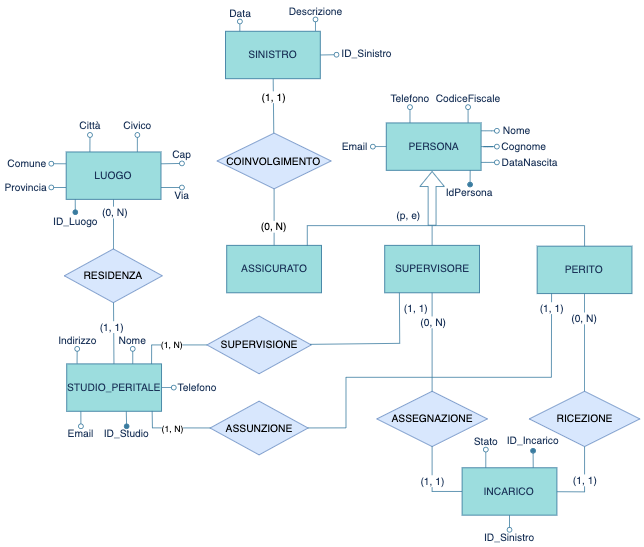
\includegraphics[width=\textwidth]{img/StudioPeritale.png}
    \end{center}
\end{figure}
\clearpage

Un \textbf{Perito}, in un determinato momento, può svolgere zero incarichi, ma anche molteplici, invece un \textbf{Incarico} può essere svolto solo da un perito.
\\
L’incarico deve per forza avere almeno una \textbf{Video Perizia} annessa (per la corretta esecuzione delle pratiche peritali), inoltre è identificato dalla combinazione di codice e perito.
\\
La video perizia può essere eseguita solo in presenza di un incarico, e quindi è identificata da un numero incrementale combinato al codice dell’incarico corrispondente.
\\
Durante la videochiamata possono essere scattate \textbf{Foto} e registrati \textbf{Video}, ma non è sempre necessario.
\\
Questi ultimi sono entità figlie di \textbf{Media}, hanno una dimensione e sono identificati dal nome e dall’estensione del file.
\\
\begin{figure}[ht]
    \begin{center}
        \centering
        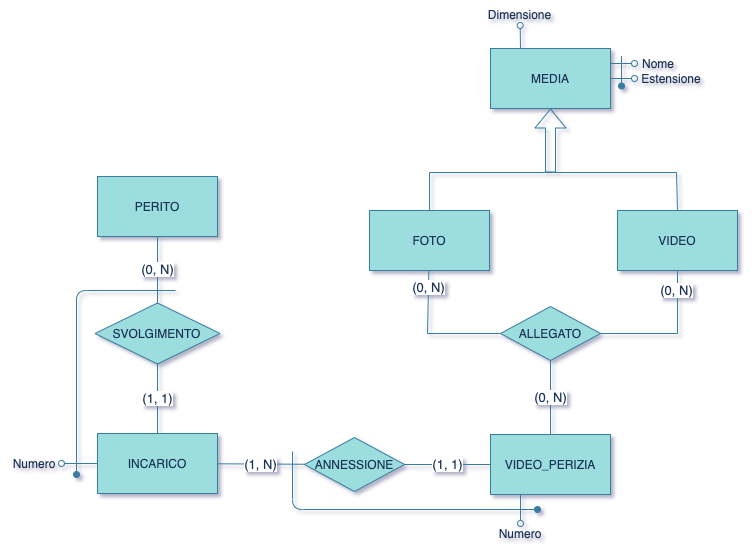
\includegraphics[width=\textwidth]{img/VideoPerizia.png}
    \end{center}
\end{figure}
\clearpage

\section{Raffinamenti proposti}

\section{Schema concettuale finale}

\begin{figure}[H]
\centering{}
\includegraphics[width=.7\textwidth]{img/observer}
\caption{Il pattern Observer è usato per consentire a GLaDOS di informare tutti i sistemi di output in ascolto}
\label{img:observer}
\end{figure}



\begin{figure}[h]
\centering{}
\includegraphics[width=\textwidth]{img/badarch}
\caption{Schema UML mal fatto e con una pessima descrizione, che non aiuta a capire. Don't try this at home.}
\label{img:badarch}
\end{figure}


\chapter{Progettazione Logica}
\section{Stima del volume dei dati}

\mbox{}\\
\def\arraystretch{2}% 
\begin{tabularx}{\textwidth}{ p{6cm} | >{\centering\arraybackslash}p{2cm} | >{\centering\arraybackslash}X }
    \textbf{Concetto} & \textbf{Costrutto} & \textbf{Volume} \\
\hline
ASSICURAZIONE & E & 30\\ \hline
EROGAZIONE & A & 2.000.000\\ \hline
POLIZZE & E & 2.000.000\\ \hline
STIPULAZIONE & A & 2.000.000\\ \hline
ASSICURATO & E & 1.000.000\\ \hline
TIPOLOGIA & A & 2.000.000\\ \hline
TIPO\_POLIZZA & E & 15\\ \hline
GENERAZIONE & A & 100.000\\ \hline
SINISTRO & E & 100.000\\ \hline
SPECIFICAZIONE & A & 100.000\\ \hline
CATEGORIA\_SINISTRO & E & 20\\
\end{tabularx}

\noindent
\def\arraystretch{2}% 
\begin{tabularx}{\textwidth}{ p{6cm} | >{\centering\arraybackslash}p{2cm} | >{\centering\arraybackslash}X }
DELEGAZIONE & A & 100.000 \\ \hline
STUDIO\_PERITALE & E & 3.000\\ \hline
DIRIGENTE & E & 4.000\\ \hline
DIREZIONE & A & 4.000\\ \hline
PERITO & E & 60.000\\ \hline
ASSUNZIONE & A & 60.000\\ \hline
ASSEGNAZIONE & E & 100.000\\ \hline
RICEZIONE & A & 100.000\\ \hline
LAVORO & A & 100.000\\
\end{tabularx}
\\
\\
\\
\\
\\
\noindent
\def\arraystretch{2}% 
\begin{tabularx}{\textwidth}{ p{6cm} | >{\centering\arraybackslash}p{2cm} | >{\centering\arraybackslash}X }
SVOLGIMENTO & A & 100.000\\ \hline
INCARICO & E & 100.000\\ \hline
FASCICOLO & A & 100.000\\ \hline
DOCUMENTI & E & 300.000\\ \hline
ANNESSIONE & A & 120.000\\ \hline
VIDEO\_PERIZIA & E & 120.000\\ \hline
ALLEGATO & A & 50.000\\ \hline
MEDIA & E & 70.000\\
\end{tabularx}

\clearpage
\section{Descrizione delle operazioni principali e stima della loro frequenza}

\def\arraystretch{2}% 
\begin{tabularx}{\textwidth}{ >{\centering\arraybackslash}p{2cm} | X |  >{\centering\arraybackslash}p{3cm} }
    \textbf{Codice} & \textbf{Operazione} & \textbf{Frequenza}\\
\hline
1 & Inserire un assicurato & 300 al giorno\\ \hline
2 & Visualizzare tutte le polizze di un assicurato & 20 al giorno\\ \hline
3 & Stipulazione di una nuova polizza tra assicurato e assicurazione & 1.000 al giorno\\ \hline
4 & Registrare un nuovo studio peritale & 15 al mese\\ \hline
5 & Rimuovere uno studio peritale & 15 al mese\\ \hline
6 & Assumere un nuovo perito o dirigente in uno studio & 5.000 all'anno\\ \hline
7 & Generare un sinistro e delegarlo a uno studio peritale & 25.000 al giorno\\ \hline
8 & Licenziare il perito di uno studio & 1.500 all'anno\\ \hline
9 & Il dirigente crea un nuovo lavoro e lo assegna a un perito & 25.000 al giorno\\ \hline
10 & Il perito crea l'incarico da svolgere in base al lavoro assegnatogli & 25.000 al giorno\\ \hline
11 & Aggiornare lo stato di un incarico & 50.000 al giorno\\
\end{tabularx}

\noindent
\def\arraystretch{2}% 
\begin{tabularx}{\textwidth}{ >{\centering\arraybackslash}p{2cm} | X |  >{\centering\arraybackslash}p{3cm} }
12 & Leggere tutti gli incarichi aperti in un determinato studio & 2.000 al giorno\\ \hline
13 & Aggiungere un documento ad un incarico & 35.000 al giorno\\ \hline
14 & Inserire una video-perizia per un incarico & 30.000 al giorno\\ \hline
15 & Allegare i media raccolti alla video-perizia & 20.000 al giorno\\ \hline
16 & Raccogliere tutte le informazioni relative a un incarico (incluse video-perizie e documenti) & 8.000 al giorno\\ \hline
17 & Visualizzare il lavoro al quale è associato un incarico & 10.000 al giorno
\end{tabularx}
\\
\\
\section{Schemi di navigazione e tabelle degli accessi}

\subsection{1 - Inserire un assicurato}
Inserire un assicurato implica che abbia stipulato un contratto con un assicurazione.
\\
\\
\def\arraystretch{2}% 
\begin{tabularx}{\textwidth}{ >{\centering\arraybackslash}p{3cm} | >{\centering\arraybackslash}X | >{\centering\arraybackslash}X |  >{\centering\arraybackslash}X }
    \textbf{Concetto} & \textbf{Costrutto} & \textbf{Accessi} & \textbf{Tipo} \\
\hline
Assicurato & E & 1 & S \\
Stipulazione & A & 1 & S \\
Polizze & E & 1 & S \\
Erogazione & A & 1 & S \\
\end{tabularx}
\begin{center}
\textbf{Totale : 4S * 300 al giorno = 2.400 al giorno}
\end{center}

\clearpage
\subsection{2 - Visualizzare tutte le polizze di un assicurato}
In media ogni assicurato avrà due polizze.
\\
\\
\def\arraystretch{2}% 
\begin{tabularx}{\textwidth}{ >{\centering\arraybackslash}p{3cm} | >{\centering\arraybackslash}X | >{\centering\arraybackslash}X |  >{\centering\arraybackslash}X }
    \textbf{Concetto} & \textbf{Costrutto} & \textbf{Accessi} & \textbf{Tipo} \\
\hline
Assicurato & E & 1 & L \\
Stipulazione & A & 1 & L \\
Polizze & E & 2 & L \\
\end{tabularx}
\begin{center}
\textbf{Totale : 4L * 20 al giorno = 80 al giorno}
\end{center}

\subsection{3 - Stipulazione di una nuova polizza tra assicurato e assicurazione}

\def\arraystretch{2}% 
\begin{tabularx}{\textwidth}{ >{\centering\arraybackslash}p{3cm} | >{\centering\arraybackslash}X | >{\centering\arraybackslash}X |  >{\centering\arraybackslash}X }
    \textbf{Concetto} & \textbf{Costrutto} & \textbf{Accessi} & \textbf{Tipo} \\
    \hline
    Stipulazione & A & 1 & S \\
    Polizze & E & 1 & S \\
    Erogazione & A & 1 & S \\
\end{tabularx}
\begin{center}
\textbf{Totale : 3S * 1.000 al giorno = 6.000 al giorno}
\end{center}
\clearpage
\subsection{4 - Registrare un nuovo studio peritale}
Inserire uno studio peritale ci vincola ad aggiungere anche almeno un dipendente e un dirigente, altrimenti lo studio non potrebbe assegnare lavori e svolgere incarichi, ciò vuol dire che si dovrà accedere in scrittura anche in Perito, Dirigente, e relative associazioni.
\\
\\
\def\arraystretch{2}% 
\begin{tabularx}{\textwidth}{ >{\centering\arraybackslash}p{3cm} | >{\centering\arraybackslash}X | >{\centering\arraybackslash}X |  >{\centering\arraybackslash}X }
    \textbf{Concetto} & \textbf{Costrutto} & \textbf{Accessi} & \textbf{Tipo} \\
    \hline
    Studio Peritale & E & 1 & S \\
    Dirigente & E & 1 & S \\
    Direzione & A & 1 & S \\
    Assunzione & A & 1 & S \\
    Perito & E & 1 & S \\
\end{tabularx}
\begin{center}
\textbf{Totale : 5S * 15 al mese = 150 al mese}
\end{center}

\clearpage
\subsection{5 - Rimuovere uno studio peritale}
Rimuovere uno studio peritale implica che non si deve tenere più traccia dei dipendenti, dei lavori e degli incarichi dello studio, inoltre, deve essere eliminata la delegazione del sinistro, in modo tale che possa essere ri-delegato a un altro studio.
\\
Uno studio peritale in media ha 33 sinistri, incarichi e lavori, 20 periti e 1 dirigente.
\\
\\
\def\arraystretch{2}% 
\begin{tabularx}{\textwidth}{ >{\centering\arraybackslash}p{3cm} | >{\centering\arraybackslash}X | >{\centering\arraybackslash}X |  >{\centering\arraybackslash}X }
    \textbf{Concetto} & \textbf{Costrutto} & \textbf{Accessi} & \textbf{Tipo} \\
    \hline
    Studio Peritale & E & 1 & S \\
    Dirigente & E & 1 & S \\
    Direzione & A & 1 & S \\
    Assunzione & A & 20 & S \\
    Perito & E & 20 & S \\
    Delegazione & A & 33 & S \\
    Incarico & E & 33 & S \\
    Svolgimento & A & 33 & S \\
    Lavoro & E & 33 & S \\
    Assegnazione & A & 33 & S \\
    Ricezione & A & 33 & S \\
\end{tabularx}
\begin{center}
\textbf{Totale : 241S * 15 al mese = 7.230 al mese}
\end{center}
\clearpage
\subsection{6 - Assumere un nuovo perito o dirigente in uno studio}
Assumere un perito o un dirigente comporta lo stesso numero di accessi per entrambe le operazioni, non c'è nessun vincolo da tenere in considerazione (a parte associarlo allo studio) quindi l'inserimento è immediato.
\\
\\
\def\arraystretch{2}% 
\begin{tabularx}{\textwidth}{ >{\centering\arraybackslash}p{3cm} | >{\centering\arraybackslash}X | >{\centering\arraybackslash}X |  >{\centering\arraybackslash}X }
    \textbf{Concetto} & \textbf{Costrutto} & \textbf{Accessi} & \textbf{Tipo} \\
    \hline
    Perito / Dirigente & E & 1 & S \\
    Assunzione / Direzione & A & 1 & S \\
\end{tabularx}
\begin{center}
\textbf{Totale : 2S * 5.000 all'anno = 20.000 all'anno}
\end{center}

\subsection{7 - Generare un sinistro e delegarlo a uno studio peritale}
Quando di genera un sinistro si deve per forza specificare anche la categoria.
\\
\\
\def\arraystretch{2}% 
\begin{tabularx}{\textwidth}{ >{\centering\arraybackslash}p{3cm} | >{\centering\arraybackslash}X | >{\centering\arraybackslash}X |  >{\centering\arraybackslash}X }
    \textbf{Concetto} & \textbf{Costrutto} & \textbf{Accessi} & \textbf{Tipo} \\
    \hline
    Generazione & A & 1 & S \\
    Sinistro & E & 1 & S \\
    Specificazione & A & 1 & S \\
    Categoria\_Sinistro & E & 1 & S \\
    Delegazione & A & 1 & S \\
\end{tabularx}
\begin{center}
\textbf{Totale : 5S * 25.000 al giorno = 250.000 al giorno}
\end{center}
\clearpage
\subsection{8 - Licenziare il perito di uno studio}
Quando si licenzia un perito lo si deve aggiornare anche nei lavori a lui assegnati e negli incarichi da lui svolti. 
\\
\\
\def\arraystretch{2}% 
\begin{tabularx}{\textwidth}{ >{\centering\arraybackslash}p{3cm} | >{\centering\arraybackslash}X | >{\centering\arraybackslash}X |  >{\centering\arraybackslash}X }
    \textbf{Concetto} & \textbf{Costrutto} & \textbf{Accessi} & \textbf{Tipo} \\
    \hline
    Perito & E & 1 & S \\
    Ricezione & A & 1 & S \\
    Svolgimento & A & 1 & S \\
    Incarico & E & 1 & S \\
\end{tabularx}
\begin{center}
\textbf{Totale : 4S * 1.500 all'anno = 12.000 all'anno}
\end{center}

\subsection{9 - Il dirigente crea un nuovo lavoro e lo assegna a un perito}

\def\arraystretch{2}% 
\begin{tabularx}{\textwidth}{ >{\centering\arraybackslash}p{3cm} | >{\centering\arraybackslash}X | >{\centering\arraybackslash}X |  >{\centering\arraybackslash}X }
    \textbf{Concetto} & \textbf{Costrutto} & \textbf{Accessi} & \textbf{Tipo} \\
    \hline
    Perito & E & 1 & S \\
    Ricezione & A & 1 & S \\
    Svolgimento & A & 1 & S \\
    Incarico & E & 1 & S \\
\end{tabularx}
\begin{center}
\textbf{Totale : 4S * 25.000 al giorno = 200.000 all'anno}
\end{center}

\clearpage
\subsection{10 - Il perito crea l'incarico da svolgere in base al lavoro assegnatogli}
L'incarico deve per forza avere annessa una video-perizia.
\\
\\
\def\arraystretch{2}% 
\begin{tabularx}{\textwidth}{ >{\centering\arraybackslash}p{3cm} | >{\centering\arraybackslash}X | >{\centering\arraybackslash}X |  >{\centering\arraybackslash}X }
    \textbf{Concetto} & \textbf{Costrutto} & \textbf{Accessi} & \textbf{Tipo} \\
    \hline
    Svolgimento & A & 1 & S \\
    Incarico & E & 1 & S \\
    Annessione & A & 1 & S \\
    Video-Perizia & E & 1 & S \\
\end{tabularx}
\begin{center}
\textbf{Totale : 4S * 25.000 al giorno = 200.000 all'anno}
\end{center}


\subsection{11 - Aggiornare lo stato di un incarico}
\\
\\
\def\arraystretch{2}% 
\begin{tabularx}{\textwidth}{ >{\centering\arraybackslash}p{3cm} | >{\centering\arraybackslash}X | >{\centering\arraybackslash}X |  >{\centering\arraybackslash}X }
    \textbf{Concetto} & \textbf{Costrutto} & \textbf{Accessi} & \textbf{Tipo} \\
    \hline
    Incarico & E & 1 & S \\
\end{tabularx}
\begin{center}
\textbf{Totale : 1S * 50.000 al giorno = 100.000 al giorno}
\end{center}

\subsection{12 - Leggere tutti gli incarichi aperti in un determinato studio}
Considerando che in media ogni studio peritale si occupa di 33 incarichi, e gli stati possono essere due (Aperto e Chiuso), avremo sempre in media 16 letture.
\\
\\
\def\arraystretch{2}% 
\begin{tabularx}{\textwidth}{ >{\centering\arraybackslash}p{3cm} | >{\centering\arraybackslash}X | >{\centering\arraybackslash}X |  >{\centering\arraybackslash}X }
    \textbf{Concetto} & \textbf{Costrutto} & \textbf{Accessi} & \textbf{Tipo} \\
    \hline
    Studio & E & 1 & L \\
    Incarico & E & 16 & L \\
\end{tabularx}
\begin{center}
\textbf{Totale : 17L * 2.000 al giorno = 34.000 al giorno}
\end{center}

\subsection{13 - Aggiungere un documento ad un incarico}
Un incarico in media include un fascicolo di 3 documenti.
\\
\\
\def\arraystretch{2}% 
\begin{tabularx}{\textwidth}{ >{\centering\arraybackslash}p{3cm} | >{\centering\arraybackslash}X | >{\centering\arraybackslash}X |  >{\centering\arraybackslash}X }
    \textbf{Concetto} & \textbf{Costrutto} & \textbf{Accessi} & \textbf{Tipo} \\
    \hline
    Incarico & E & 1 & L \\
    Documenti & E & 3 & S \\
    Fascicolo & A & 3 & S \\
\end{tabularx}
\begin{center}
\textbf{Totale : (1L + 6S) * 35.000 al giorno = 26.000 al giorno}
\end{center}

\subsection{14 - Inserire una video-perizia per un incarico}

\def\arraystretch{2}% 
\begin{tabularx}{\textwidth}{ >{\centering\arraybackslash}p{3cm} | >{\centering\arraybackslash}X | >{\centering\arraybackslash}X |  >{\centering\arraybackslash}X }
    \textbf{Concetto} & \textbf{Costrutto} & \textbf{Accessi} & \textbf{Tipo} \\
    \hline
    Video-Perizia & E & 1 & S \\
    Annessione & A & 1 & S \\
\end{tabularx}
\begin{center}
\textbf{Totale : 2S * 30.000 al giorno = 120.000 al giorno}
\end{center}

\subsection{15 - Allegare i media raccolti alla video-perizia}
In media, per ogni allegato ci sono due media.
\\
\\
\def\arraystretch{2}% 
\begin{tabularx}{\textwidth}{ >{\centering\arraybackslash}p{3cm} | >{\centering\arraybackslash}X | >{\centering\arraybackslash}X |  >{\centering\arraybackslash}X }
    \textbf{Concetto} & \textbf{Costrutto} & \textbf{Accessi} & \textbf{Tipo} \\
    \hline
    Media & E & 2 & S \\
    Allegato & A & 2 & S \\
\end{tabularx}
\begin{center}
\textbf{Totale : 2S * 20.000 al giorno = 120.000 al giorno}
\end{center}

\subsection{16 - Raccogliere tutte le informazioni relative a un  incarico (incluse video-perizie e documenti)}
In media ogni incarico ha 1 video-perizia annessa e 3 documenti allegati.
\\
\\
\def\arraystretch{2}% 
\begin{tabularx}{\textwidth}{ >{\centering\arraybackslash}p{3cm} | >{\centering\arraybackslash}X | >{\centering\arraybackslash}X |  >{\centering\arraybackslash}X }
    \textbf{Concetto} & \textbf{Costrutto} & \textbf{Accessi} & \textbf{Tipo} \\
    \hline
    Incarico & E & 1 & L \\
    Video-Perizia & E & 1 & L \\
    Annessione & A & 1 & L \\
    Documento & E & 3 & L \\
    Fascicolo & A & 3 & L \\
\end{tabularx}
\begin{center}
\textbf{Totale : 9L * 8.000 al giorno = 72.000 al giorno}
\end{center}

\subsection{17 - Visualizzare il lavoro al quale è visualizzato un incarico}

\def\arraystretch{2}% 
\begin{tabularx}{\textwidth}{ >{\centering\arraybackslash}p{3cm} | >{\centering\arraybackslash}X | >{\centering\arraybackslash}X |  >{\centering\arraybackslash}X }
    \textbf{Concetto} & \textbf{Costrutto} & \textbf{Accessi} & \textbf{Tipo} \\
    \hline
    Incarico & E & 1 & L \\
    Lavoro & E & 1 & L \\
\end{tabularx}
\begin{center}
\textbf{Totale : 2L * 10.000 al giorno = 20.000 al giorno}
\end{center}

\clearpage
\section{Raffinamento dello schema}

\subsection{Eliminazione delle gerarchie}
Per l’eliminazione della gerarchia Persona si è scelto di adottare l’approccio del collasso verso il basso, replicando così gli attributi in Assicurato, Dirigente e Perito.
Si è adottata questa strategia in quanto si ha la necessità di trattare nello specifico ogni tipo di persona dando rilievo al ruolo di ognuna, per esempio bisogna ben diversificare i ruoli di Dirigente e Perito.
\\
\subsection{Eliminazione degli attributi composti}
Nello schema ER è presente un unico attributo composto, posto nell’entità Sinistro, ovvero Luogo, che è stato reso  un entità portandosi dietro i suoi sotto-componenti.
Sarà poi necessario accertarsi, a livello applicativo che tali attributi coesistano senza dar luogo a incoerenze (Esempio: non potranno esistere luoghi con un cap non corrispondente a quello della città).
\\
\subsection{Scelta delle chiavi primarie}
Nello schema sono già evidenziate senza ambiguità tutte le chiavi primarie per la maggior parte delle entità; per quanto riguarda le entità della gerarchia persona, si sceglie di usare come chiave primaria, la chiave composta da un codice e un codice fiscale per riuscire a gestire anche i casi di omocodia.
\\
Inoltre per l’entità Perito si ha una chiave alternativa utile ad associare con coerenza sinistri, lavori, e i relativi incarichi.
\clearpage
\subsection{Eliminazione degli identificatori esterni}
Dallo schema principale sono state eliminate le seguenti relazioni:
\begin{itemize}
    \item \textbf{Stipulazione}, importando ID\_Assicurato in Polizze
    \item \textbf{Erogazione}, importando Denominazione in Polizze
    \item \textbf{Generazione}, importando Denominazione in Sinistro
    \item \textbf{Delegazione}, importando ID\_Studio in Sinistro
    \item \textbf{Assunzione}, importando Codice in Studio\_Peritale
    \item \textbf{Ricezione}, importando Codice in Lavoro
    \item \textbf{Svolgimento}, importando Codice in Incarico
    \item \textbf{Annessione}, importando Codice e Numero in Video\_Perizia
\end{itemize}

\section{Analisi delle ridondanze}
\section{Traduzione di entità e associazioni in relazioni}
\section{Schema relazionale finale}
\section{Traduzione delle operazioni in query SQL}

\chapter{Progettazione dell'applicazione}
\section{Autovalutazione e lavori futuri}
\section{Difficoltà incontrate e commenti per i docenti}

\end{document}
